\newpage

\appendix
\section{Appendices}


\section{Model convergence}
\label{appendix:model_convergence}

\begin{figure}[H] 
    \centering
    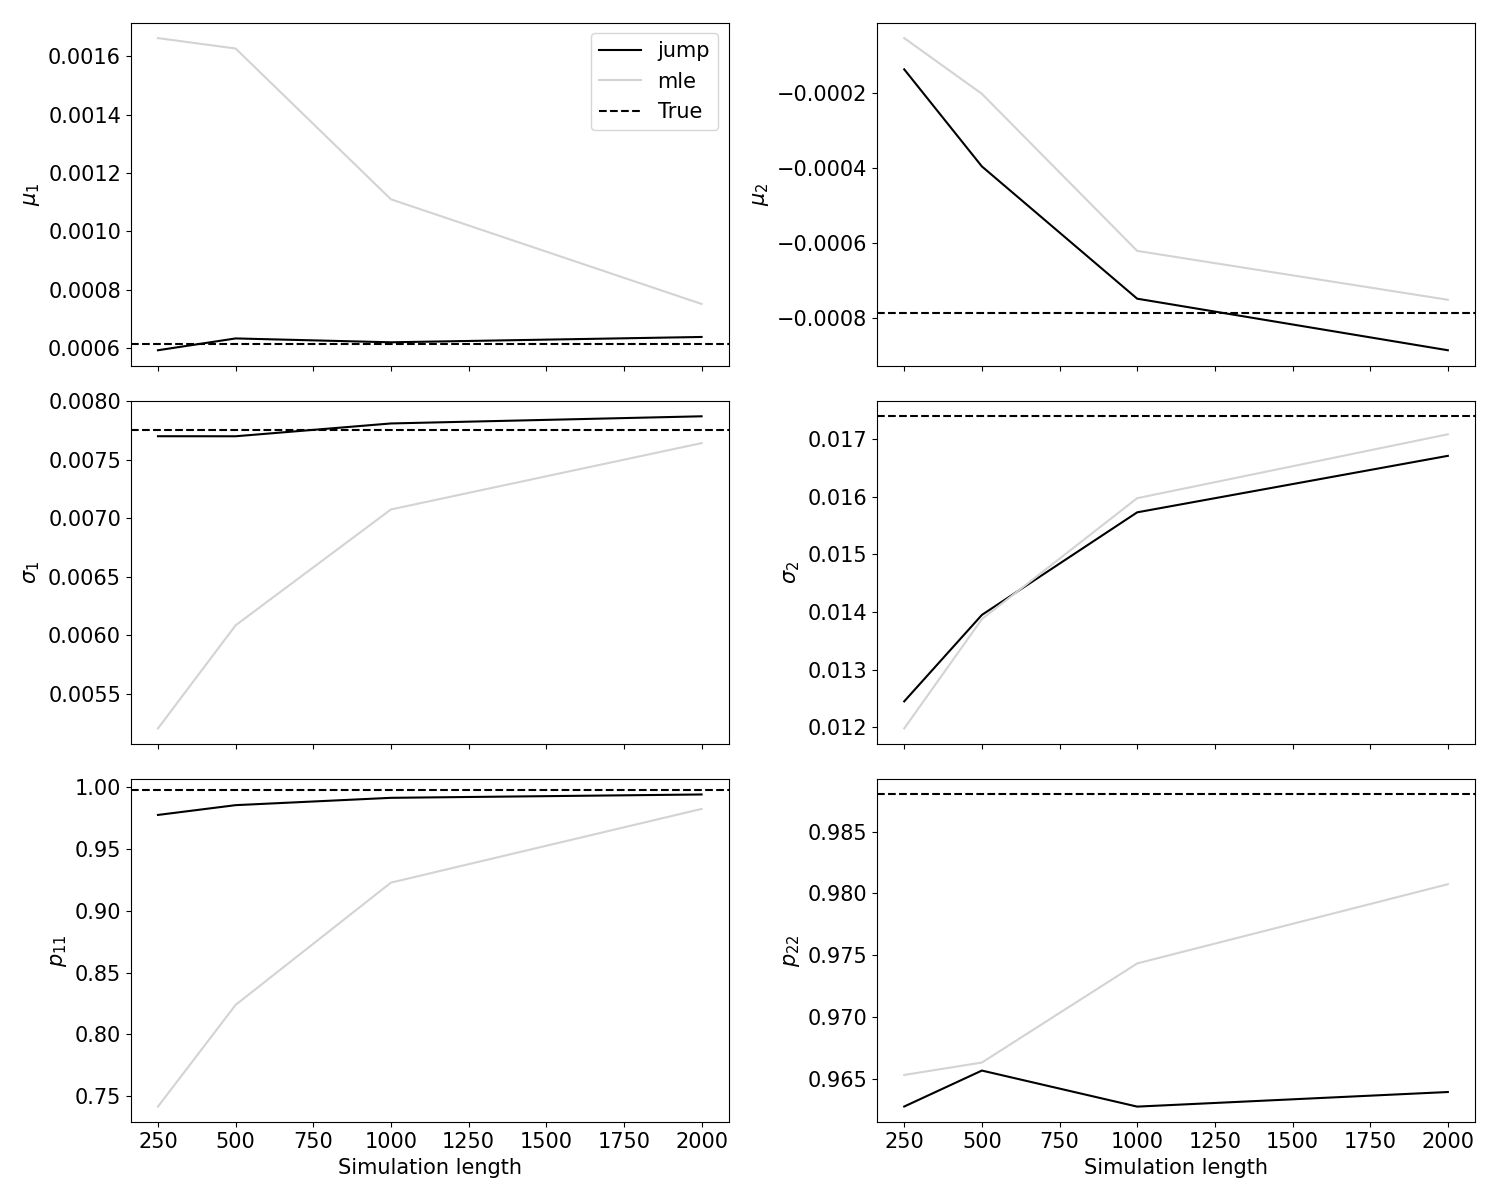
\includegraphics[width=1\textwidth]{analysis/model_convergence/images/simulation_normal.png}
    \caption{Estimates of HMM models' convergence towards true values as a function of simulation length. Results are based on 1000 simulations from conditional gaussian distributions.}
    \label{fig:jump_normal}
\end{figure}

\begin{figure}[H] 
    \centering
    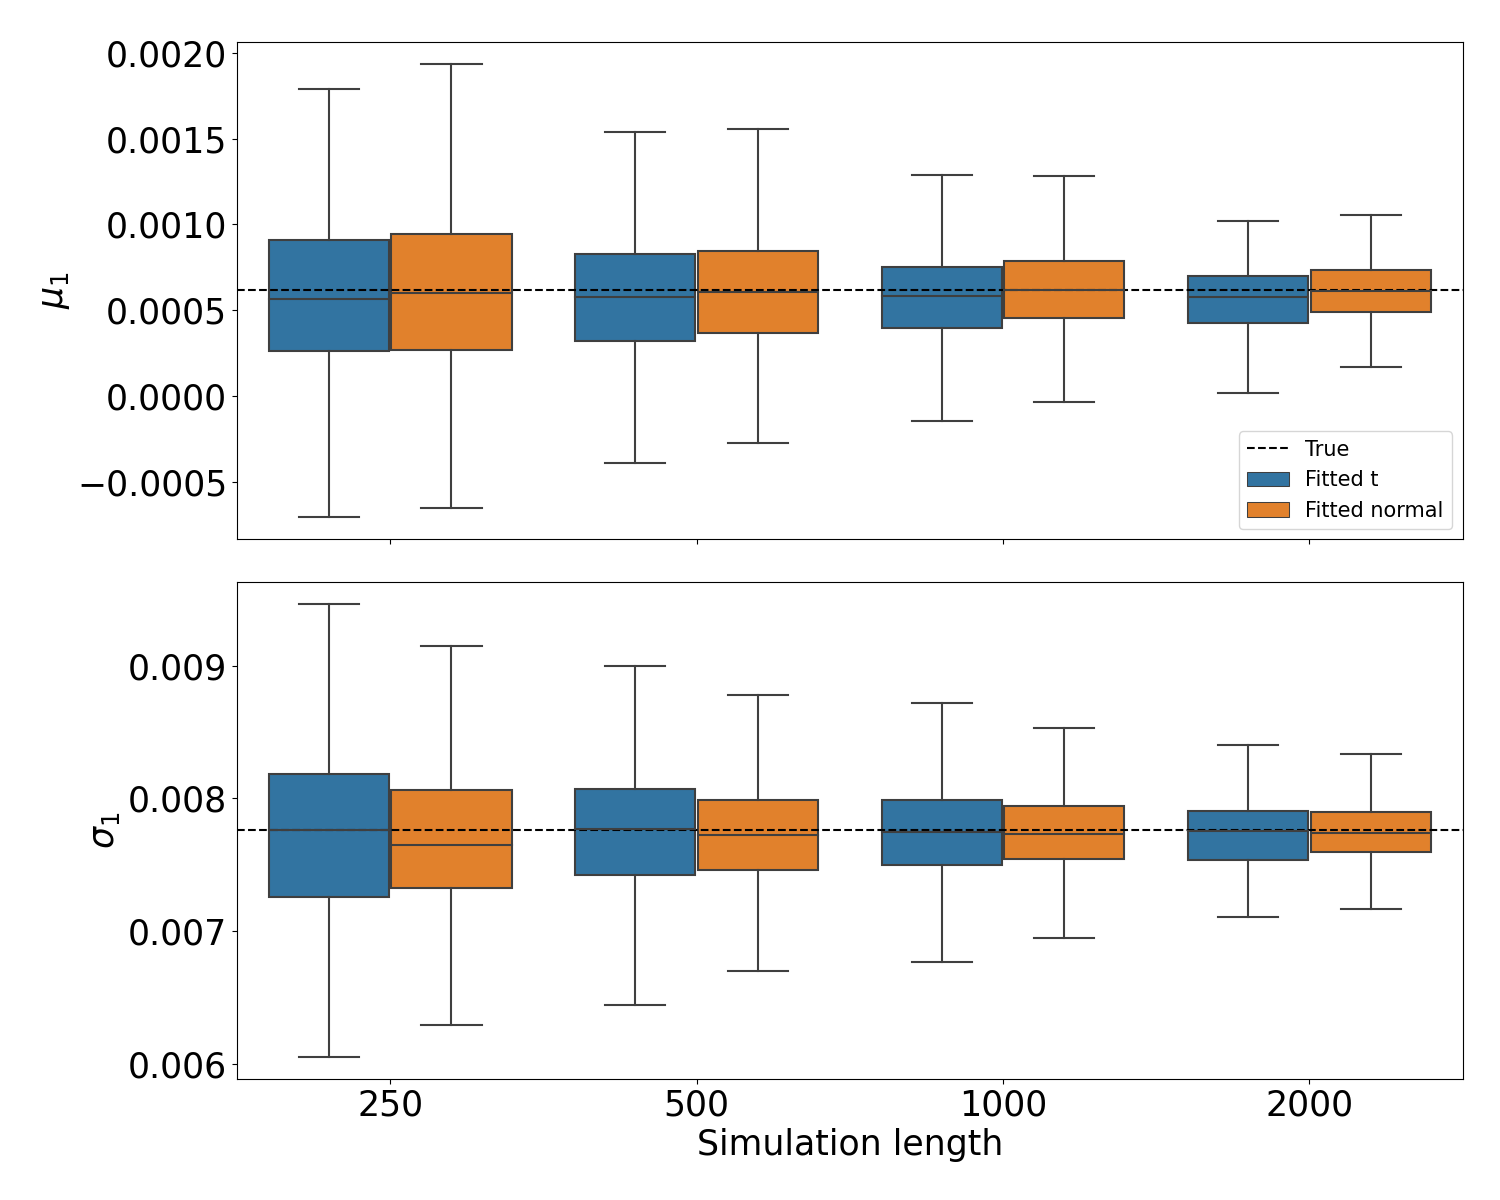
\includegraphics[width=1\textwidth]{analysis/model_convergence/images/theoretical_fit_t_dist.png}
    \caption{Empirical fit of a normal and t-distribution to data simulated from a t distribution with five degrees of freedom. Results are based on 1000 simulated series.}
    \label{fig:jump_theoretical_fit}
\end{figure}

\begin{figure}[H] 
    \centering
    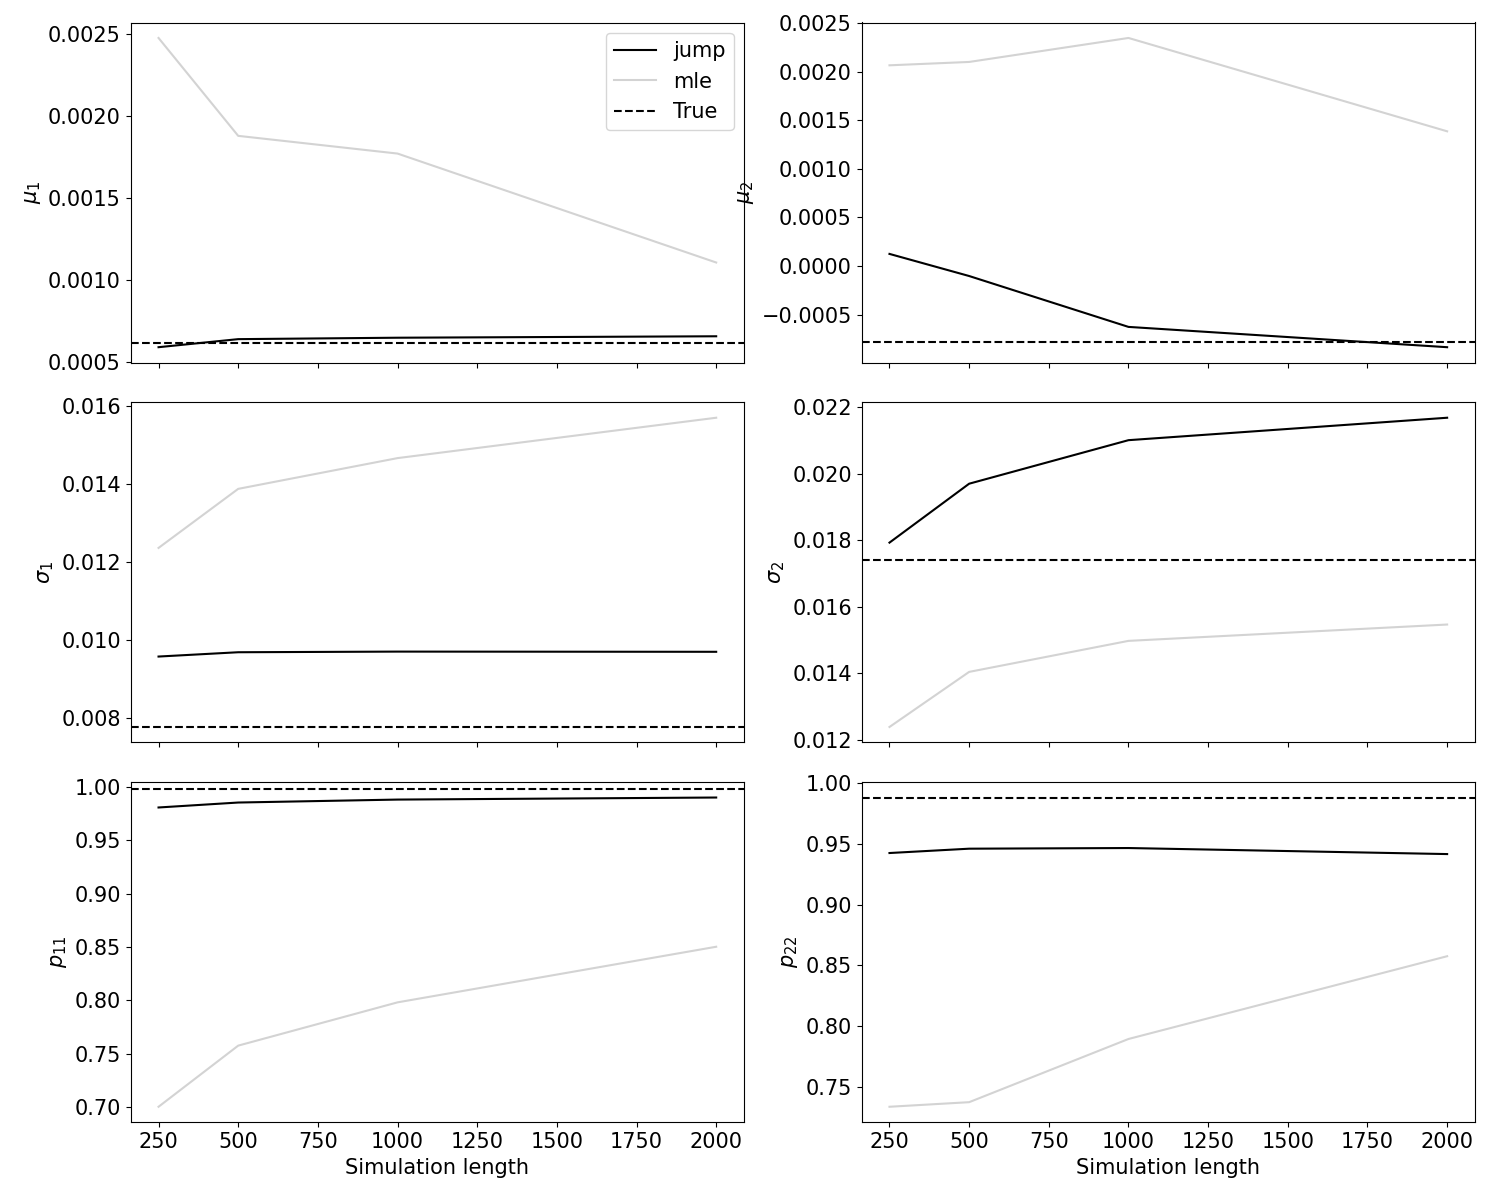
\includegraphics[width=1\textwidth]{analysis/model_convergence/images/simulation_t.png}
    \caption{Estimates of HMM models' convergence towards true values as a function of simulation length. Results are based on 1000 simulations with conditional t distributions with five degrees of freedom.}
    \label{fig:jump_t}
\end{figure}

\section{Box-plot of jump penalties}
\label{appendix:box_plot}

\begin{figure}[H] 
    \centering
    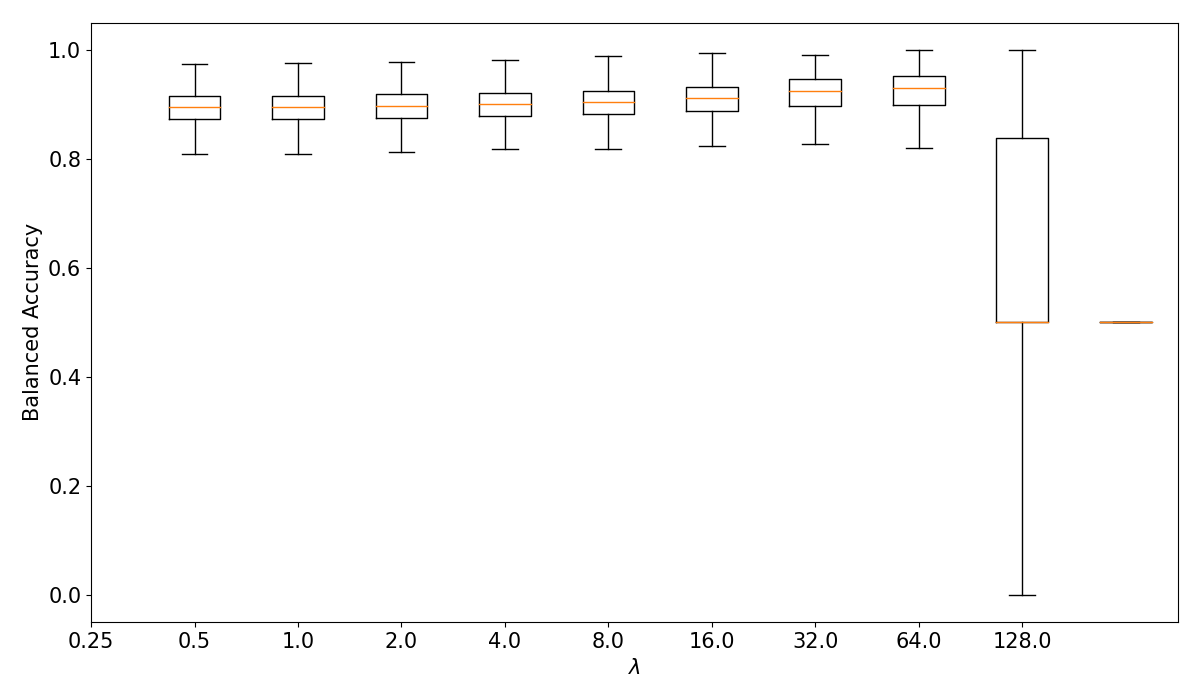
\includegraphics[width=1\textwidth]{analysis/model_convergence/images/jump_penalties_box.png}
    \caption{Hyper-tuning.}
    %\label{fig:jump_penalties}
\end{figure}


\section{Outlier corrected rolling moments}

\begin{figure}[H] 
    \centering
    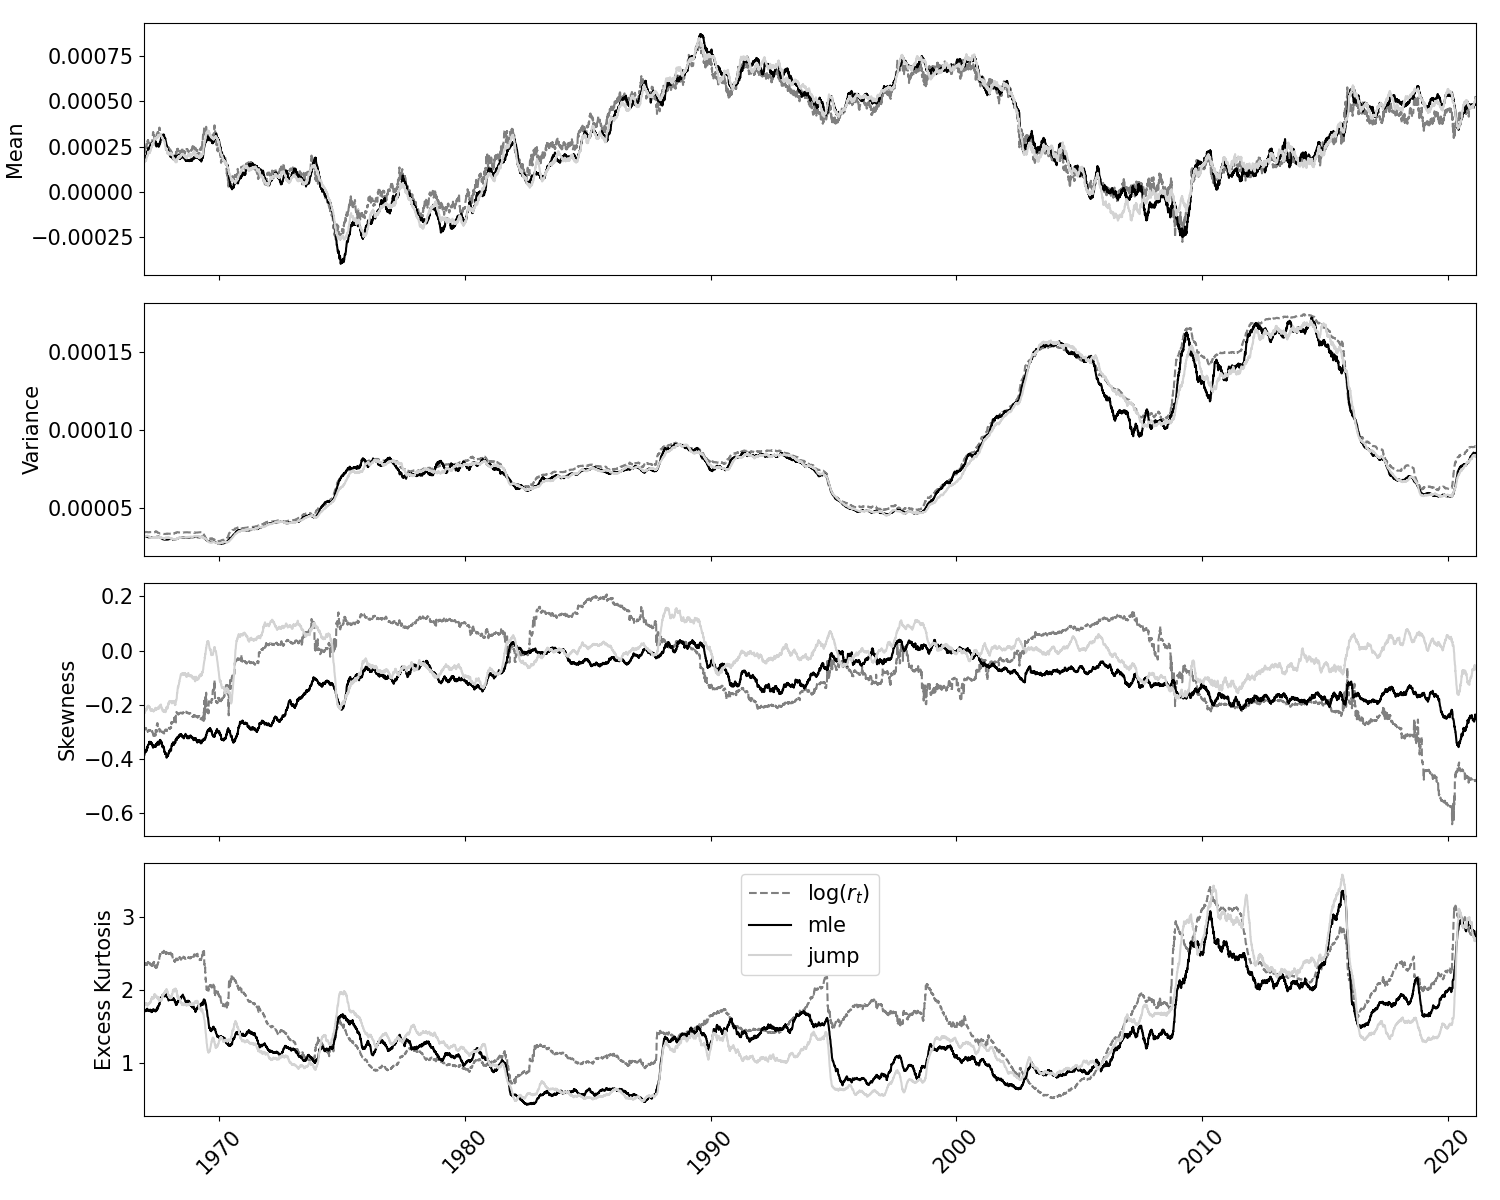
\includegraphics[width=1.0\textwidth]{analysis/stylized_facts/images/moments_outlier_corrected.png}
    \caption{Development of first four moments of estimated models compared to $\log(r_t)$ using a rolling window of 1700 days and correcting for outliers that are further than four standard deviations away from the mean. Outliers are treated locally in each subsample of 1700 observations. Model estimates are calculated using Monte-Carlo simulations.}
\end{figure}
\label{fig:stylized_facts_rolling_moments_outliers_appendix}



